\documentclass["../Cours.tex"]{subfiles}
\usepackage{multirow}

\begin{document}

{ \color{noir}

\setcounter{probleme}{1}
\probleme{Dessins complexes}

\begin{questions}

\PARTIETITRE{Carte de France}

\textit{Dans cette partie, nous allons voir comment dessiner une carte de France, en utilisant le quadrillage du cahier.}

\question Construire la structure suivante :

\begin{center}
    \begin{tikzpicture}[scale=0.6]
        \draw[thin,gray!40!white] (0,0) grid (14,13);
        \draw[Latex-Latex] (0,-0.5) -- +(14,0) node[midway,below]{14 carreaux};
        \draw[Latex-Latex] (14.5,0) -- +(0,13) node[midway,right]{13 carreaux};
        \draw (8,13) -- (8,0);
        \draw (0,10) -- (14,10);
        \draw (7,12) -- (8,12);
        \draw (3,10) -- +(0,1.5);
        \draw (3,2) -- +(10,0);
        \draw (11,2) -- +(0,-1);
        \fill (8,10) circle (0.1) node[above right]{$O(0;0)$};
    \end{tikzpicture}
\end{center}

\question \textbf{Nord-ouest : } Suivre les étapes ci-dessous

\begin{center}
    \begin{tikzpicture}[scale=0.4]
        \draw[thin,gray!40!white] (0,0) grid (14,13);
        \draw[rouge] (8,13) -- (8,0);
        \draw[rouge] (0,10) -- (14,10);
        \draw[rouge] (7,12) -- (8,12);
        \draw[rouge] (3,10) -- +(0,1.5);
        \draw[rouge] (3,2) -- +(10,0);
        \draw[rouge] (11,2) -- +(0,-1);
        \draw[very thick] (8,13) arc (90:180:1);
    \end{tikzpicture}
    \begin{tikzpicture}[scale=0.4]
        \draw[thin,gray!40!white] (0,0) grid (14,13);
        \draw[rouge] (8,13) -- (8,0);
        \draw[rouge] (0,10) -- (14,10);
        \draw[rouge] (7,12) -- (8,12);
        \draw[rouge] (3,10) -- +(0,1.5);
        \draw[rouge] (3,2) -- +(10,0);
        \draw[rouge] (11,2) -- +(0,-1);
        \draw[very thick] (8,13) arc (90:180:1);
        \draw[very thick] (7,12) .. controls (7,11.5) and (4,10) .. (4,11.5) -- (3,11.5);
    \end{tikzpicture}
    \begin{tikzpicture}[scale=0.4]
        \draw[thin,gray!40!white] (0,0) grid (14,13);
        \draw[rouge] (8,13) -- (8,0);
        \draw[rouge] (0,10) -- (14,10);
        \draw[rouge] (7,12) -- (8,12);
        \draw[rouge] (3,10) -- +(0,1.5);
        \draw[rouge] (3,2) -- +(10,0);
        \draw[rouge] (11,2) -- +(0,-1);
        \draw[very thick] (8,13) arc (90:180:1);
        \draw[very thick] (7,12) .. controls (7,11.5) and (4,10) .. (4,11.5) -- (3,11.5) -- (3,10) -- (0,10);
    \end{tikzpicture}
\end{center}

\clearpage
\question \textbf{Sud-ouest : } Suivre les étapes ci-dessous

\begin{center}
    \begin{tikzpicture}[scale=0.4]
        \draw[thin,gray!40!white] (0,0) grid (14,13);
        \draw[rouge] (8,13) -- (8,0);
        \draw[rouge] (0,10) -- (14,10);
        \draw[rouge] (7,12) -- (8,12);
        \draw[rouge] (3,10) -- +(0,1.5);
        \draw[rouge] (3,2) -- +(10,0);
        \draw[rouge] (11,2) -- +(0,-1);
        \draw[very thick] (0,10) -- (0,9) .. controls (4,8) and (4,2) .. (3,2);
    \end{tikzpicture}
    \begin{tikzpicture}[scale=0.4]
        \draw[thin,gray!40!white] (0,0) grid (14,13);
        \draw[rouge] (8,13) -- (8,0);
        \draw[rouge] (0,10) -- (14,10);
        \draw[rouge] (7,12) -- (8,12);
        \draw[rouge] (3,10) -- +(0,1.5);
        \draw[rouge] (3,2) -- +(10,0);
        \draw[rouge] (11,2) -- +(0,-1);
        \draw[very thick] (0,10) -- (0,9) .. controls (4,8) and (4,2) .. (3,2);
        \draw[very thick] (3,2) .. controls (3,0) and (8,0) .. (8,0);
    \end{tikzpicture}
\end{center}

\question \textbf{Sud-est : } Suivre les étapes ci-dessous

\begin{center}
    \begin{tikzpicture}[scale=0.4]
        \draw[thin,gray!40!white] (0,0) grid (14,13);
        \draw[rouge] (8,13) -- (8,0);
        \draw[rouge] (0,10) -- (14,10);
        \draw[rouge] (7,12) -- (8,12);
        \draw[rouge] (3,10) -- +(0,1.5);
        \draw[rouge] (3,2) -- +(10,0);
        \draw[rouge] (11,2) -- +(0,-1);
        \draw[very thick] (8,0) .. controls (8,2) and (11,1) .. (11,1);
    \end{tikzpicture}
    \begin{tikzpicture}[scale=0.4]
        \draw[thin,gray!40!white] (0,0) grid (14,13);
        \draw[rouge] (8,13) -- (8,0);
        \draw[rouge] (0,10) -- (14,10);
        \draw[rouge] (7,12) -- (8,12);
        \draw[rouge] (3,10) -- +(0,1.5);
        \draw[rouge] (3,2) -- +(10,0);
        \draw[rouge] (11,2) -- +(0,-1);
        \draw[very thick] (8,0) .. controls (8,2) and (11,1) .. (11,1);
        \draw[very thick] (11,1) .. controls (11,0.5) and (12,0.5) .. (13,2);
    \end{tikzpicture}
\end{center}

\question \textbf{Nord-est : } Suivre les étapes ci-dessous

\begin{center}
    \begin{tikzpicture}[scale=0.4]
        \draw[thin,gray!40!white] (0,0) grid (14,13);
        \draw[rouge] (8,13) -- (8,0);
        \draw[rouge] (0,10) -- (14,10);
        \draw[rouge] (7,12) -- (8,12);
        \draw[rouge] (3,10) -- +(0,1.5);
        \draw[rouge] (3,2) -- +(10,0);
        \draw[rouge] (11,2) -- +(0,-1);
        \draw[very thick] (13,2) .. controls (12,4) and (12,8) .. (14,10);
    \end{tikzpicture}
    \begin{tikzpicture}[scale=0.4]
        \draw[thin,gray!40!white] (0,0) grid (14,13);
        \draw[rouge] (8,13) -- (8,0);
        \draw[rouge] (0,10) -- (14,10);
        \draw[rouge] (7,12) -- (8,12);
        \draw[rouge] (3,10) -- +(0,1.5);
        \draw[rouge] (3,2) -- +(10,0);
        \draw[rouge] (11,2) -- +(0,-1);
        \draw[very thick] (13,2) .. controls (12,4) and (12,8) .. (14,10);
        \draw[very thick] (14,10) .. controls (13,10) and (9,12) .. (8,13);
    \end{tikzpicture}
\end{center}

\question Sur la carte de France obtenue, 
    \subquestion Placer les villes suivantes : Paris, Marseille, Brest, Lille, Strasbourg, Bordeaux
    \subquestion Pour chacune de ces villes, donner leur coordonnées sur la carte.

\question \textbf{Pour aller plus loin : }
    \subquestion Placer d'autres villes sur la carte.
    \subquestion Avec un crayon de couleur bleu, dessiner les principaux fleuves de France.

\clearpage
\PARTIETITRE{Patron d'une jupe}

\question \textit{La Haute Autorité de Santé (HAS) explique comment mesurer le tour de taille et son lien avec l'obésité. }
\begin{flushright}\vspace{-2ex}
    \tiny{(source : https://www.has-sante.fr/upload/docs/application/pdf/2011-12/recommandation\_obesite\_adulte.pdf)}
\end{flushright}

\begin{center}
    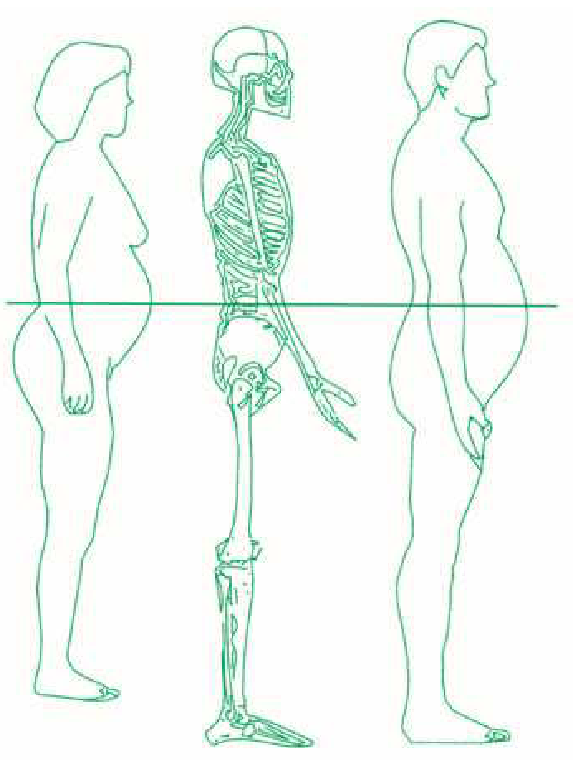
\includegraphics[scale=0.25]{4 - Quatrieme/problemes/Screenshot_20230524_033734.png}
\end{center}

\textit{Le diagnostic de surpoids et d’obésité repose sur l’indice de masse corporelle (IMC) calculé à partir du poids (en kilogrammes) et de la taille (en mètres) (poids/taille au carré).}

\textit{Pour un IMC égal ou supérieur à \qty{25}{\kg\per\metre\squared} et inférieur à \qty{35}{\kg\per\metre\squared}, l’examen clinique devra être complété par la mesure du tour de taille à mi-distance entre la dernière côte et le sommet de la crête iliaque} 

\textit{Le tour de taille est un indicateur simple de l’excès de graisse au niveau abdominal chez l’adulte (obésité abdominale). L’excès de graisse abdominale est associé, indépendamment de l’IMC, au développement des complications métaboliques et vasculaires de l’obésité.}

\textit{Il n’y a aucun argument pour inciter à perdre du poids un patient en simple surpoids stable et sans comorbidité associée, mais il est important de prévenir une prise de poids supplémentaire.}

\begin{center}
    \begin{tabularx}{0.8\linewidth}{*{4}{|C}|}\hline
        \multirow{2}{*}{\makecell{IMC\\(\unit{\kg\per\metre\squared})}} & \multicolumn{2}{|c|}{\makecell{Tour de taille \\(\unit{\cm})}} & \multirow{2}{*}{\makecell{Présence de\\ comorbidité}} \\\cline{2-3}
         & \makecell{Bas \\ hommes $< 94$ \\ femmes $<80$} & \makecell{Élevé \\ hommes $\supeg 94$ \\ femmes $\supeg 80$} & \\\hline
        25-30 & Surpoids simple & Surpoids avec tour de taille élevé & \cellcolor{gray} \\\hline
        30-35 & \cellcolor{gray} & \cellcolor{gray} & \cellcolor{gray} \\\hline
        35-40 & \cellcolor{gray} & \cellcolor{gray} & \cellcolor{noir} \\\hline 
        $>40$ & \cellcolor{noir} & \cellcolor{noir} & \cellcolor{noir} \\\hline
    \end{tabularx}
\end{center}


\begin{tikzpicture}[baseline=(current bounding box.south)]
    \fill[gray] (0,0) rectangle (2,0.3);
\end{tikzpicture}
Intervention proposée : réduire le poids de \qty{5}{\%} à \qty{15}{\%}.

\begin{tikzpicture}[baseline=(current bounding box.south)]
    \fill[noir] (0,0) rectangle (2,0.3);
\end{tikzpicture}
Intervention proposée : réduire le poids / considérer la chirurgie bariatrique.

    \subquestion Qu'est-il recommandé pour un patient en surpoids simple ? 
    \subquestion Un médecin prend les mesures et pèse un patient. Il s'agit d'un homme d'1m75 pesant \qty{88}{\kilo\gram} et ayant un tour de taille de \qty{102}{\cm}. Il n'a pas de comorbidité. Que faut-il lui recommander ?
    \subquestion À partir de quelle valeur considère-t-on un tour de taille élevé pour une femme ?

\clearpage
\question \textbf{Prises des mesures}
    \subquestion À l'aide d'une corde ou d'un ruban-mètre, mesurer le tour de taille.
    \subquestion Mesurer le tour de hanches (la zone la plus large située sur le bas du corps).
    \subquestion Déterminer la longueur de la jupe (mesurer à partir de la taille puis descendre jusqu'à la longueur de jupe souhaitée).

\medskip
\textit{Dans la suite du problème, par défaut, on choisira :
\begin{itemize}
    \item tour de taille : $t = \qty{67}{\centi\metre}$
    \item tour de hanches : $h = \qty{96}{\centi\metre}$
    \item longueur de la jupe : $l = \qty{45}{\centi\metre}$
\end{itemize}}

\bigskip
\centerline{\textbf{TOUTES LES CONSTRUCTIONS SUR FEUILLE SERONT À L'ÉCHELLE 1/10.}}
\bigskip

\question \textbf{Construction du patron}
    \subquestion Construire un rectangle de longueur $h/2+\num{1.5}$ et de hauteur $l$.
    \subquestion \scalebox{0.9}[1]{Tracer un segment horizontal $[CD]$ sur toute la longueur du rectangle à \qty{9}{\centi\metre} du haut du rectangle.}
    \subquestion \scalebox{0.9}[1]{Tracer un segment horizontal $[EF]$ sur toute la longueur du rectangle à \qty{22}{\centi\metre} du haut du rectangle.}
    \subquestion Placer $A$ le milieu du côté haut du rectangle, et $B$ le milieu du côté bas du rectangle ; tracer $[AB]$.

\question \textbf{Construction du patron : les pinces}
    \subquestion 
    \begin{itemize}
        \item La pince du milieu a pour dimension $p_1 = (h/2+\num{1.5})-(t/2+\num{1.5})-8$.
        \item Construire un segment horizontal $[PP']$ de longueur $p_1$ centré au point $A$.
        \item $[AB]$ et $[EF]$ sont sécants en $P''$. Tracer le triangle $PP'P''$.
    \end{itemize} 
    \subquestion 
    \begin{itemize}
        \item Placer les points $Q$ et $Q'$ respectivement à \qty{8}{\cm} et \qty{10}{\cm} du coin supérieur gauche du rectangle. 
        \item Construire la médiatrice de $[QQ']$.
        \item La médiatrice et $[CD]$ sont sécants en $Q''$. Tracer le triangle $QQ'Q''$.
    \end{itemize}
    \subquestion 
    \begin{itemize}
        \item Placer $R$ à \qty{1}{\cm} à gauche du milieu de $[Q'P]$ et $R'$ à \qty{1}{\cm} à droite du milieu de $[Q'P]$.
        \item Construire la médiatrice de $[RR']$.
        \item La médiatrice et $[CD]$ sont sécants en $R''$. Tracer le triangle $RR'R''$.
    \end{itemize}
    \subquestion Placer S à \qty{1}{\cm} à gauche du coin supérieur droit ; tracer $[SF]$.
    \subquestion 
    \begin{itemize}
        \item Placer $T$ à \qty{1.5}{\cm} à gauche du milieu de $[P'S]$ et $T'$ à \qty{1.5}{\cm} à droite du milieu de $[P'S]$.
        \item Construire la médiatrice de $[TT']$.
        \item La médiatrice et $[EF]$ sont sécants en $T''$. Tracer le triangle $TT'T''$.
    \end{itemize}
\end{questions}

}

\end{document}